\subsection{Overordnet}\label{sec:evaOverordnet}

% Magnus
\textbf{Møder på DTU:} Gruppen har mødtes dagligt, både i planlægnings-, implementerings- og rapportskrivningensfasen. Den første uge brugte vi en storskærm i 324, så alle kunne følge med i den grundlæggende kodes tilblivelse linje for linje. \\

% Magnus
% Hvordan holdt I styr på projektet?  Logbog.
\textbf{Logbog:} For at holde styr på projektets status, har vi ført logbog flere gange dagligt i \texttt{Google Docs}. Logbogen er nu på 10 sider, og rummer oversigter over: Hvad er for nyligt blevet implementeret eller debugged? Hvad skal implementeres eller debugges fremover? Logbogen benytter også farvekoder; Features der skal implementeres er farvet rød. Når de er implementeret, farves de grønne. Vi har også noteret når fx metoder skifter funktionalitet, eller variable har fået nyt navn for at øge læsbarheden af koden.\\

\begin{figure}[H]
\centering
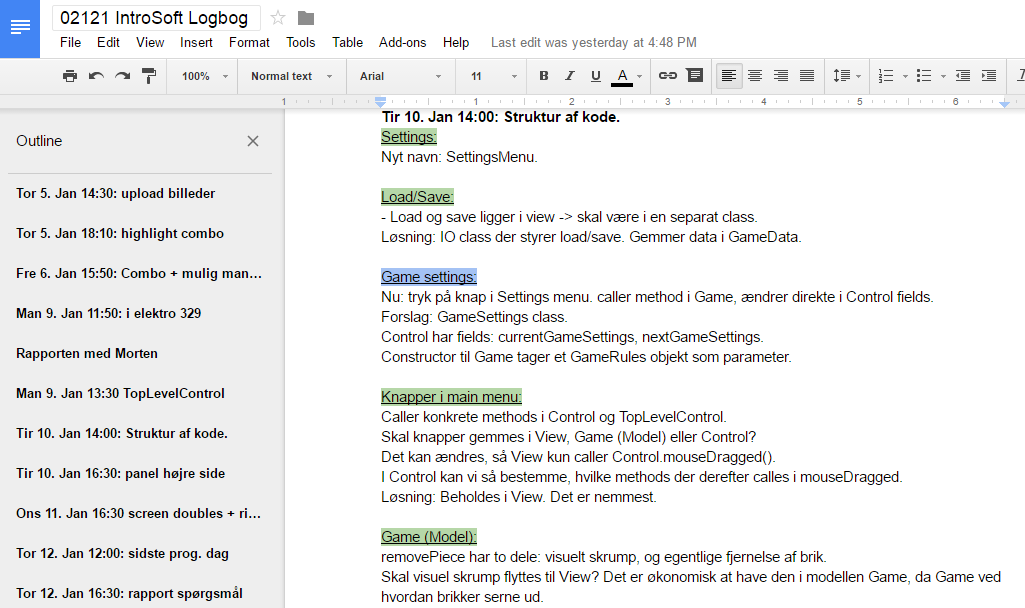
\includegraphics[width = 0.7  \textwidth]{Figurer/logbog.png}
\caption{Udsnit af den brugte logbog i løbet af projektet. Logbogen indeholder ting der skulle huskes, ting der er blevet implementeret, eller ideer til fremtidige implementeringer til programmet.}
\label{fig:logbog}
\end{figure}

% Magnus
\textbf{Sammenligning med andres spil:} For at få overblik over, hvad der adskiller vores program fra de andre gruppers, har vi besøgt andre grupper og spillet deres spil. De har spillet vores spil, og vi har spillet deres. Vi har stillet dem spørgsmål om implementering, og de har stillet os spørgsmål. Svarene på deres spørgsmål er inkorporeret i rapporten. \\

% Magnus
\textbf{100 spørgsmål:} For at sikre, at vi fik forklaret alle væsentlige dele af programmets design og implementering, stillede vi 100 spørgsmål, fx: Hvordan flytter spilleren en brik? Hvordan ændres brætstørrelsen? Hvordan highlightes felter?
Vi tog derefter udgangspunkt i, at rapporten skulle besvare alle spørgsmål. På den måde forsøgte vi at dokumentere programmet fyldestgørende. 